\documentclass{beamer}
\usepackage{beamerthemesplit}
\usepackage{color}
\usepackage{amsfonts}
\usepackage{multimedia}
\usepackage{animate}
\usepackage{wrapfig}
\usepackage{multicol}
%\setlength{\textwidth}{15cm}           %Sets the width of the printable area of the page to 15cm
%\setlength{\topmargin}{0cm}            %Space from the toprule to the top of the text (first line) to 0 cm.
%\setlength{\footskip}{0cm}               %Space from the bottom of the text to the footnote (or footrule) to 0 cm.
\setlength{\marginparwidth}{0cm}   
\setlength{\columnsep}{0cm}
%\newlist{arrowlist}{itemize}{1}
%\setlist[arrowlist]{label=$\Rightarrow$}


\definecolor{cvggreen}{RGB}{4,71,79}
\mode<presentation>
{
%Darmstadt
\usetheme[compress]{Amsterdam}
}
\title{Marchiatura digitale di sequenze video stereoscopiche a disparit\`{a} coerente }
\author{Benedetta Barbetti,\\ 
		Michaela Servi}
\institute{Universit\`{a} degli studi di Firenze}
\date{10 Dicembre 2015}


\begin{document}

\begin{frame}
\titlepage
\end{frame}

\begin{section}{Introduzione}
\subsection{Video Stereoscopici}

\begin{frame}[t]{\textsc{Contesto}}
\centering
Numerose applicazioni di elaborazione di immagini e video richiedono esplicite informazioni sulla \textbf{profondit\`{a}} della scena. La \textbf{stereoscopia} permette di ottenere queste informazioni.
\setlength{\columnsep}{0cm}
\begin{columns}
\begin{column}{4cm}
\begin{center}
\setbeamertemplate{blocks}[rounded][shadow=false]
	\setbeamercolor{block body}{use=structure,fg=black,bg=lightgray} 	
\begin{block}{Campi applicativi}
		\begin{itemize}
			\item \small{Medicina} 
			\item Robotica
			\item Tracking
			\item Industria manifatturiera
			\item Cinema
		\end{itemize}	
	\end{block}
\end{center}
\end{column}
\begin{column}{6cm}
\begin{figure}
\centering
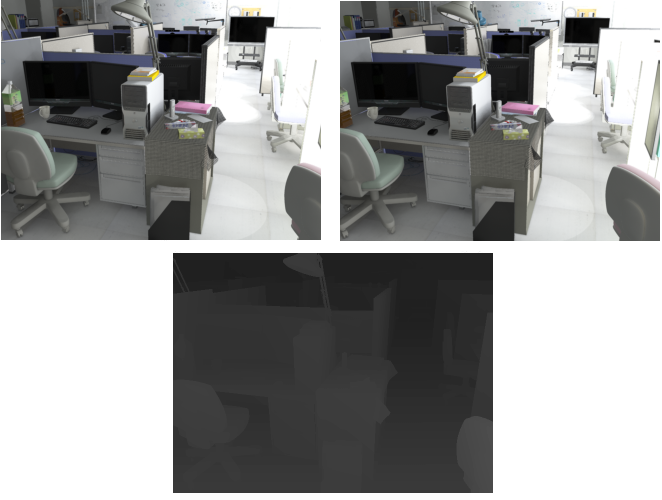
\includegraphics[width=1\linewidth]{./img/track.png}
\end{figure}
\end{column}
\end{columns}
\end{frame}


% % % % % % % % % % FRAME % % % % % % % % % % % % %

\begin{frame}[t]{\textsc{Stereoscopia}}
\vspace{-1em}
\begin{center}
	\setbeamertemplate{blocks}[rounded][shadow=false]
	\setbeamercolor{block title}{use=structure,fg=black,bg=lightgray} 
	\setbeamercolor{block body}{use=structure,fg=black,bg=lightgray} 		
\begin{block}{}
	\center Tecnica di realizzazione e visione di immagini e filmati, atta a trasmettere una illusione di \textbf{tridimensionalit\`{a}}
	\end{block}
\end{center}
\begin{center}
\vspace{-0.3em}
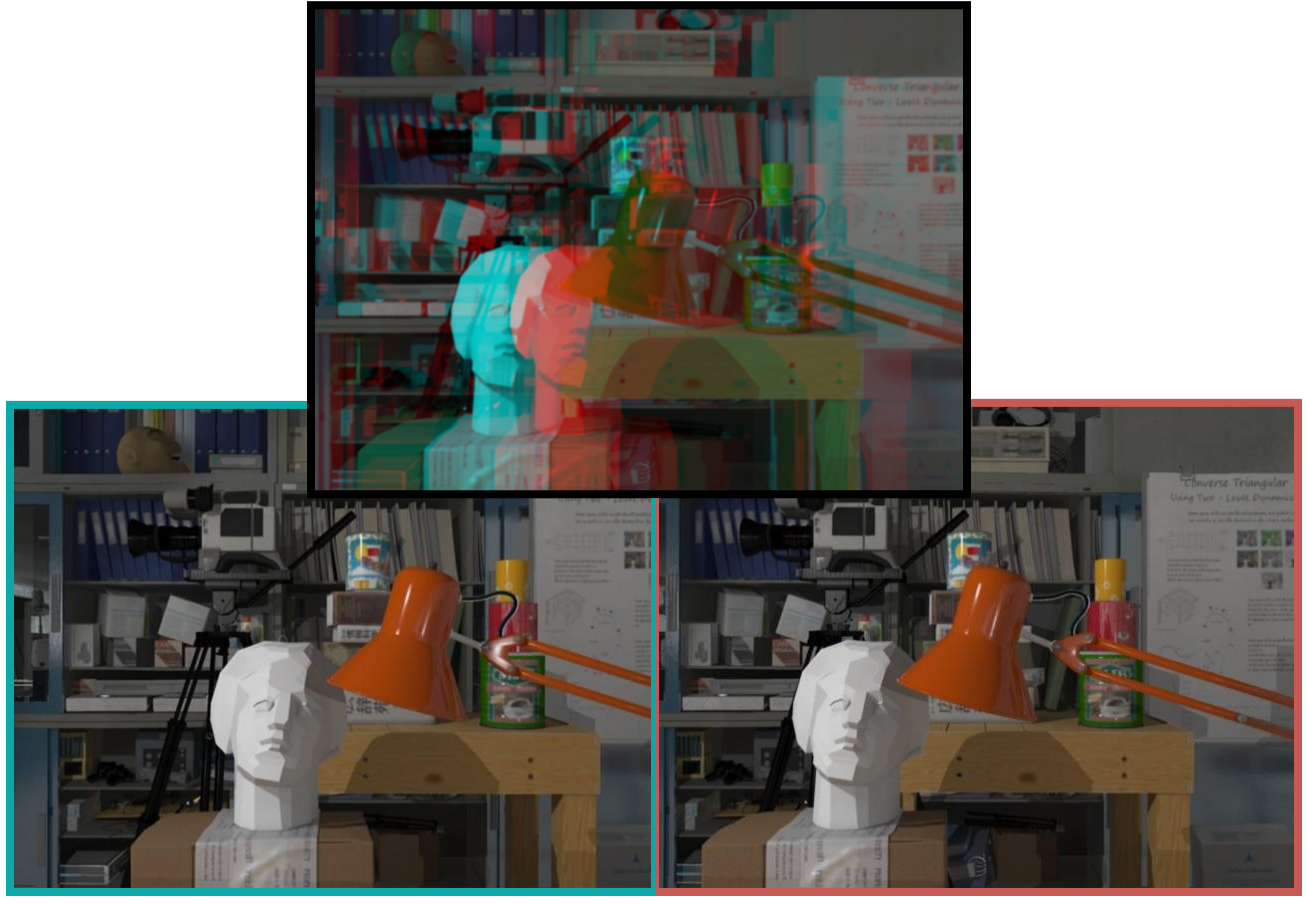
\includegraphics[width=0.7\linewidth]{./img/stereo.png}
\end{center}
\end{frame}


% % % % % % % % % % FRAME % % % % % % % % % % % % %


\begin{frame}[t]{\textsc{Video Stereoscopici}}
\setbeamertemplate{blocks}[rounded][shadow=false]
\setbeamercolor{block title}{use=structure,fg=black,bg=lightgray} 
\setbeamercolor{block body}{use=structure,fg=black,bg=lightgray} 	
	\vspace{-0.5em}
	\begin{center}
		\setbeamertemplate{blocks}[rounded][shadow=false]
		\setbeamercolor{block title}{use=structure,fg=black,bg=lightgray} 
		\setbeamercolor{block body}{use=structure,fg=black,bg=lightgray} 		
	\begin{block}{}
		\center Il \textbf{video stereoscopico} \`{e} ottenuto inquadrando la stessa scena da due \textbf{punti di vista diversi}
		\end{block}
	\end{center}
\begin{center}
\movie[width=8cm,height=5cm,autostart,loop,poster]{}{./img/alice.mp4}
\end{center}
\end{frame}

% % % % % % % % % % FRAME % % % % % % % % % % % % %

\begin{frame}[t]{\textsc{Dispositivi di ripresa e visualizzazione}}
\vspace{-0.3em}
\begin{columns}
\begin{column}{5cm}
\begin{center}
\setbeamertemplate{blocks}[rounded][shadow=false]
	\setbeamercolor{block body}{use=structure,fg=black,bg=lightgray} 
	\setbeamerfont{block body}{size=\tiny}	
\begin{block}{Sistema di ripresa stereo}
		\begin{itemize}
			\item  \small{Due telecamere sincronizzate
			\item Correttamente allineate
			\item Stessi parametri}
		\end{itemize}	
	\end{block}
\end{center}
\centering
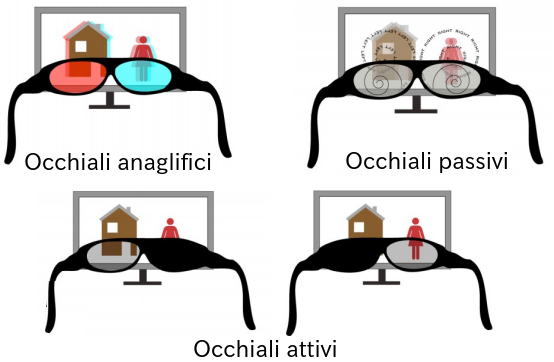
\includegraphics[width=1\linewidth]{./img/display.png}
\end{column}
\begin{column}{5cm}
\centering
\vspace{0.7em}
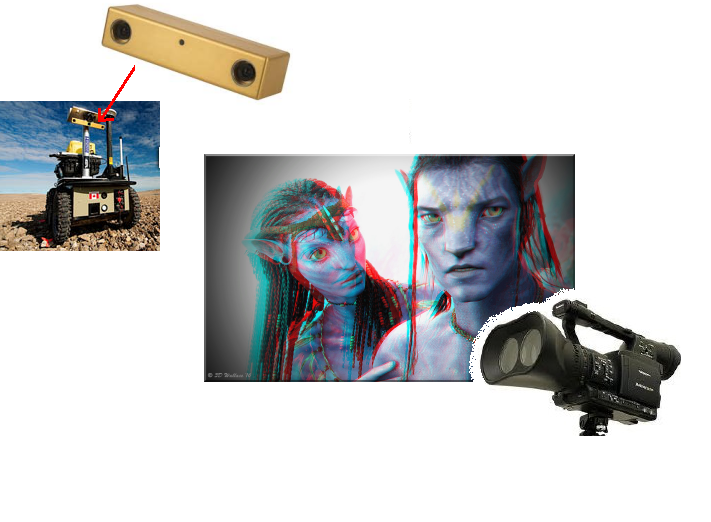
\includegraphics[width=1\linewidth]{./img/camere.png}
\vspace{-2.8em}
\begin{center}
\setbeamertemplate{blocks}[rounded][shadow=false]
	\setbeamercolor{block body}{use=structure,fg=black,bg=lightgray} 		
\begin{block}{Sistema di riproduzione}
		\begin{itemize}
			\item  \small{\textbf{Attivo}: lenti sincronizzate con il televisore
			\item \textbf{Passivo}: lenti diversamente polarizzate
			\item \textbf{Anaglifico}: lenti passive con filtri di colore diverso}
		\end{itemize}	
	\end{block}
\end{center}
\end{column}
\end{columns}
\end{frame}

% % % % % % % % % % FRAME % % % % % % % % % % % % %


\begin{frame}[t]{\textsc{Necessit\`{a} di una marchiatura}}
\setbeamertemplate{blocks}[rounded][shadow=false]
%\setbeamercolor{block title}{use=structure,fg=black,bg=lightgray} 
\setbeamercolor{block body}{use=structure,fg=black,bg=lightgray} 
\begin{columns}[T]
\begin{column}[T]{5cm}
\begin{center}
\begin{block}{Generalmente}
\begin{itemize}
\item  Sicurezza
\item  Copyright
\end{itemize}
\end{block}
\end{center}
\end{column}
\begin{column}[T]{5cm}
\begin{figure}
  
\includegraphics[width=1\textwidth]{./img/download.jpg}
  \label{fig:rna_binding}
\end{figure}
\end{column}
\end{columns}
\begin{block}{Per i contenuti 3D}
\begin{itemize}
\item Cercare una soluzione pi\`{u} adatta alla particolarit\`{a} dei contenuti
\item Scarsit\`{a} di soluzioni in letteratura
\end{itemize}
\end{block}
\end{frame}

% % % % % % % % % % FRAME % % % % % % % % % % % % %


\begin{frame}[t]{\textsc{Scopo di questa tesi}}
\vspace{2em}

\begin{itemize}
\item \textbf{Algoritmo di marchiatura a disparit\`{a} coerente nel dominio spaziale}
\end{itemize}
\begin{itemize}
\item \textbf{Algoritmo di marchiatura a disparit\`{a} coerente nel dominio della frequenza
}
\end{itemize}
\begin{center}
	\setbeamertemplate{blocks}[rounded][shadow=false]
	\setbeamercolor{block title}{use=structure,fg=black,bg=lightgray} 
	\setbeamercolor{block body}{use=structure,fg=black,bg=lightgray}
\begin{block}{}
\center \small{Watermarking \textbf{a disparit\`{a} coerente}: un punto fisico della scena ripresa deve \textit{portare} lo stesso campione di watermark indipendentemente che esso appaia nella vista sinistra o destra }
\end{block}
\end{center}
\end{frame}




\end{section}

\begin{section}{Concetti base}
\subsection{Principi della stereoscopia}

\begin{frame}[t]{\textsc{Background}}
\begin{columns}
\begin{column}{5cm}
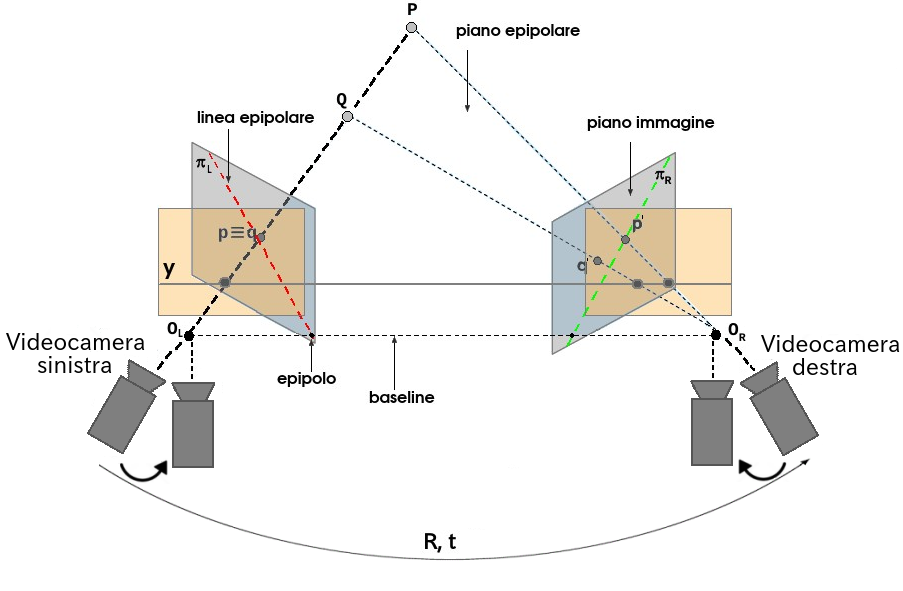
\includegraphics[width=1.1\linewidth]{./img/rect.png}
\begin{itemize}
\item[1.] \small{Calibrazione parametri intriseci ed estrinseci
\item[2.] Rettificazione
\item[3.] Calcolo delle corrispondenze
\item[4.] Computazione mappa di disparit\`{a}}
\end{itemize}
\end{column}
\begin{column}{5cm}
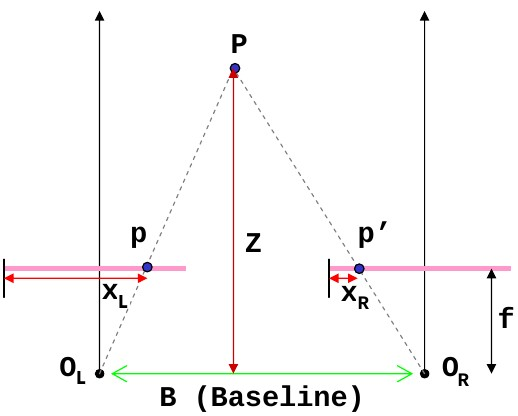
\includegraphics[width=0.8\linewidth]{./img/depth.jpg}
\begin{itemize}
\item \small{Triangolazione}:
\begin{center}
 $\frac{B}{Z} = \frac{(B+x_{L}) - x_{R}}{Z-f}$,
$Z = \frac{B \cdot f}{x_{L} - x_{R}} = \frac{B \cdot f}{d}$
\end{center}
\item  $ d = x_{L} - x_{R} $ \`{e} la disparit\`{a} 
\end{itemize}
\end{column}
\end{columns}
\end{frame}


% % % % % % % % % % FRAME % % % % % % % % % % % % %


\begin{frame}[t]{\textsc{Mappa di Disparit\`{a}: codifica}}
\begin{columns}
\hspace*{-4em}
\begin{column}{5cm}
\vspace{1em}
\begin{itemize}
\item  Codificata come un'immagine in scala di grigi
\item  Punti pi\`{u} vicini alla telecamera sono pi\`{u} chiari e corrispondono a una disparit\`{a} maggiore 
\end{itemize}
\end{column}
\hspace*{-3em}
\begin{column}{5.5cm}
\vspace{2em}
\centering
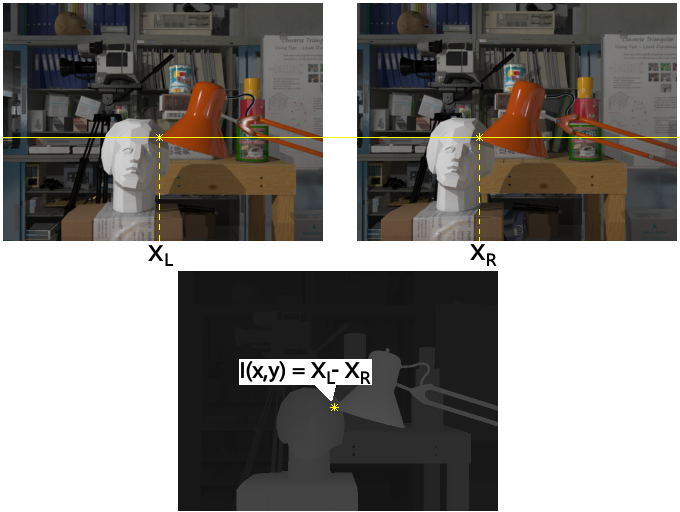
\includegraphics[width=1.2\linewidth]{./img/disparity.png}
\end{column}
\end{columns}
\end{frame}


% % % % % % % % % % FRAME % % % % % % % % % % % % %


\begin{frame}[t]{\textsc{Mappa di Disparit\`{a}: computazione}}
\begin{columns}
\begin{column}{5cm}
\vspace{1em}
\begin{itemize}
\item \small{\textbf{Metodi locali}: calcolare un valore di similarit\`{a} (MSE, NCC..) all'interno di una finestra  
\item \textbf{Metodi globali}: minimizzare su tutta l'immagine una funzione di energia che racchiude le assunzioni di corrispondenza
}
\end{itemize}
\end{column}
\begin{column}{5.5cm}
\vspace{1.5em}
\centering
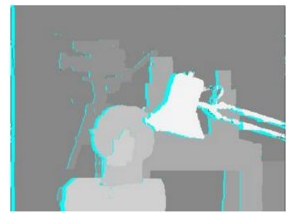
\includegraphics[width=1\linewidth]{./img/graph.png}
\end{column}
\end{columns}
\vspace{-1em}
\begin{center}
	\setbeamertemplate{blocks}[rounded][shadow=false]
	\setbeamercolor{block title}{use=structure,fg=black,bg=lightgray} 
	\setbeamercolor{block body}{use=structure,fg=black,bg=lightgray}
\begin{block}{}
\center \small{In questa tesi \`{e} stato utilizzato l'algoritmo di Kolmogorov and Zabih \textbf{Graph Cuts Stereo Matching Algorithm}}
\end{block}
\end{center}
\end{frame}


% % % % % % % % % % FRAME % % % % % % % % % % % % %


\subsection {Principi del watermarking}
\begin{frame}[t]{\textsc{Watermarking}}
\begin{columns}
\begin{column}{5cm}
\vspace{1em}
%	\setbeamertemplate{blocks}[rounded][shadow=false]
%	\setbeamercolor{block title}{use=structure,fg=black,bg=lightgray} 
%	\setbeamercolor{block body}{use=structure,fg=black,bg=lightgray}
%\begin{block}{}
%\center \small{Il \textbf{watermarking digitale} consiste nell'\textbf{inserimento} di \textbf{informazione} in contenuti  multimediali digitali in modo tale che questa informazione possa essere successivamente \textbf{estratta} o individuata per investigare possibili \textbf{manipolazioni} del contenuto ed eventuali violazioni del \textbf{copyright}}
%\end{block}
\textbf{Processo di marchiatura}
\begin{itemize}
\item Codifica di informazione nascosta in un contenuto originale
\item Distribuzione del contenuto
\item Ritrovamento del marchio
\end{itemize}
\textbf{Propriet\`{a}}
\begin{itemize}
\item Trasparenza
\item Robustezza
\end{itemize}
\end{column}
\begin{column}{5cm}
\centering
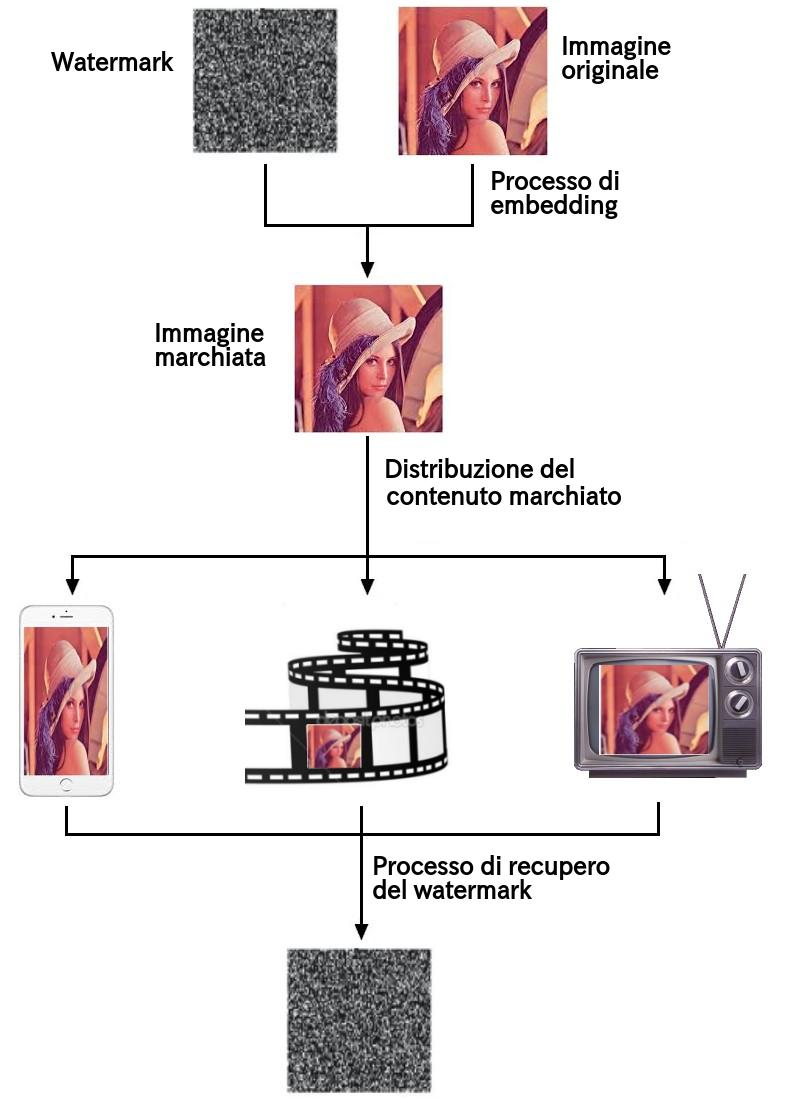
\includegraphics[width=1\linewidth]{./img/wat_workflow.jpg}
\end{column}
\end{columns}
\end{frame}

%\begin{frame}[t]{\textsc{Nozioni generali}}
%\begin{columns}
%\begin{column}{5cm}
%\vspace{1em}
%	\setbeamertemplate{blocks}[rounded][shadow=false]
%	\setbeamercolor{block body}{use=structure,fg=black,bg=lightgray}
%\begin{block}{Classificazione delle tecniche}
%\begin{itemize}
%\item Blind/Non blind
%\item Privata/Pubblica
%\item A lettura/A rilevamento
%\end{itemize}
%\end{block}
%\end{column}
%\begin{column}{5cm}
%\vspace{1em}
%	\setbeamertemplate{blocks}[rounded][shadow=false]
%	\setbeamercolor{block body}{use=structure,fg=black,bg=lightgray}
%\begin{block}{Requisiti del watermark}
%\begin{itemize}
%\item Trasparenza
%\item Robustezza
%\item Capacit\`{a}
%\end{itemize}
%\end{block}
%\end{column}
%\end{columns}
%\vspace{1em}
%\setbeamertemplate{blocks}[rounded][shadow=false]
%\setbeamercolor{block body}{use=structure,fg=black,bg=lightgray}
%\begin{block}{Domini e tecniche di inserimento}
%\begin{itemize}
%\item Spaziale/ Frequenza(DFT, DCT, DWT)
%\item Spread Spectrum/ Side Information
%\end{itemize}
%\end{block}
%\end{frame}

\subsection{Robustezza}
\vspace{2em}
\begin{frame}[t]{\textsc{View Synthesis}}
	\setbeamertemplate{blocks}[rounded][shadow=false]
	\setbeamercolor{block title}{use=structure,fg=black,bg=lightgray} 
	\setbeamercolor{block body}{use=structure,fg=black,bg=lightgray}
\begin{block}{}
\center \small{ Dato un insieme di immagini della stessa scena ottenute da diversi punti di vista, una \textbf{nuova immagine} viene \textbf{creata} considerando una \textbf{camera virtuale} posizionata in un diverso punto dello spazio}
\end{block}
\vspace{2em}
\centering
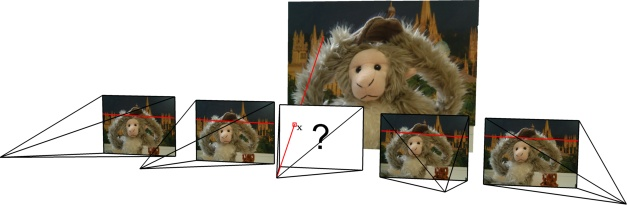
\includegraphics[width=1\linewidth]{./img/nvs.jpg}
\end{frame}

%\subsection{Tecniche di inserimento}
%\vspace{1em}
%\begin{frame}[t]{\textsc{Spread Spectrum nel dominio spaziale}}
%\begin{columns}
%\begin{column}{5cm}
%	\setbeamertemplate{blocks}[rounded][shadow=false]
%	\setbeamercolor{block body}{use=structure,fg=black,bg=lightgray}
%\vspace{1em}
%\begin{block}{Codifica}
%\centering Un pattern di rumore pseudo-random viene sommato al valore di luminanza di tutti i pixel dell'immagine
%$ \mathbf{I_{w}(x,y) = I(x,y) + \alpha w(x,y)}$
%\end{block}
%\begin{block}{Detection}
%Data l'immagine $\mathbf{I'}$ ritenuta marchiata viene calcolata la correlazione con il marchio $\mathbf{w}$
%\end{block}
%\end{column}
%\begin{column}{5cm}
%\vspace{1.5em}
%\centering
%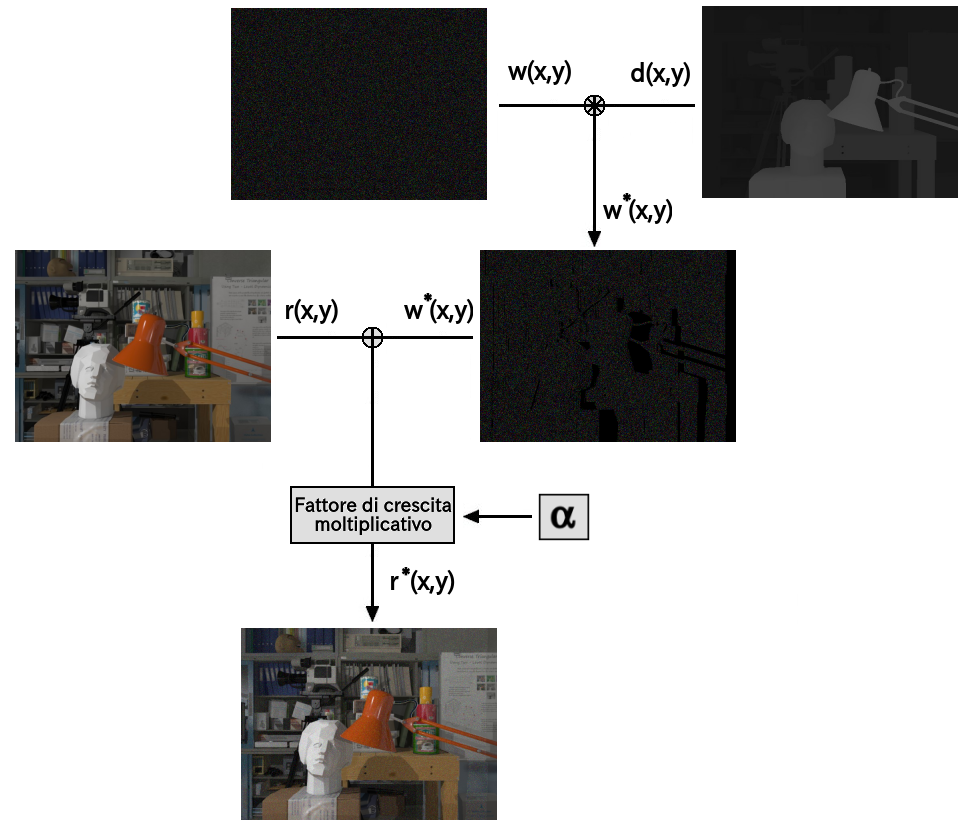
\includegraphics[width=1\linewidth]{./img/ss.png}
%\end{column}
%\end{columns}
%\end{frame}
%
%
%\subsection{Domini di inserimento}
%\begin{frame}[t]{\textsc{Inserimento in DFT}}
%\vspace{1em}
%\centering
%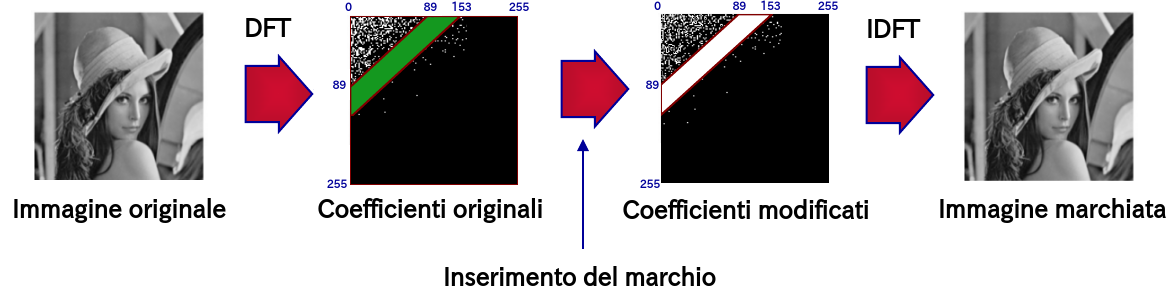
\includegraphics[width=1\linewidth]{./img/dft.png}
%\begin{itemize}
%\item Trasformazione immagine con Discrete Fourier Transform
%\item Selezione di n coefficienti $\mathbf{v_i}$ (medie frequenze)
%\item Generazione di una sequenza pseudo-random $\mathbf{w}$
%\item Modifica dei coefficienti: 
%\vspace{-2.3em}
% \begin{align*} 
%\qquad \mathbf{v'_{i} = v_i + \alpha w_{i}}\\
%		\mathbf{v'_{i} = v_i + \alpha v_i  w_{i}}
%\end{align*}
%\vspace{-2.5em}
%\item Ritorno al dominio spaziale con la trasformata inversa
%\end{itemize}
%\end{frame}

\subsection{Watermarking di video stereoscopici}

% % % % % % % % % % FRAME % % % % % % % % % % % % %


\begin{frame}[t]{\textsc{Metodi a Disparit\`{a} Coerente}}
\vspace{1em}
\centering

\begin{center}
\begin{itemize}

\item Marchiatura della \textbf{coppia stereo}
\item \textbf{Punti corrispondenti} nelle due viste presentano lo \textbf{stesso} campione del \textbf{marchio}
\item Il watermark viene modificato in base alla disparit\`{a} prima di essere inserito nella vista destra 
\item Vantaggi:
	\begin{itemize}
	\item Migliore \textbf{qualit\`{a} visiva}
	\item Maggior grado di \textbf{robustezza} contro attacchi di \textbf{view synthesis}
	\end{itemize}
\end{itemize}
\end{center}
\end{frame}
 
 
 % % % % % % % % % % FRAME % % % % % % % % % % % % %

\end{section}

\begin{section}{Marchiatura spaziale}
\subsection{Processo di codifica}
\begin{frame}[t]{\textsc{Marchiatura spaziale a disparit\`{a} coerente}}
\vspace{-2em}
\begin{columns}
\begin{column}{6cm}
	\setbeamertemplate{blocks}[rounded][shadow=false]
	\setbeamercolor{block body}{use=structure,fg=black,bg=lightgray}
\vspace{1em}
\begin{block}{Codifica vista sinistra}
\begin{itemize}
\item Metodo Spread Spectrum(\textbf{SS}):
\begin{center}
$\mathbf{l^{w} = l+\alpha w_{K}}$
\end{center}
\item Il marchio $\mathbf{w_{K}}$ segue $\sim N(0, 1)$, $\alpha \in \{1,3\}$
\end{itemize}
\end{block}
\begin{block}{Codifica vista destra}
\begin{itemize}
\item $\mathbf{w_{K}}$ deformato in base ai valori della disparit\`{a}:
\begin{center}
 $\mathbf{w^{*}_{K}(x,y) = w_{K}(x+d(x,y), y)}$
\end{center}
\item Inserito con SS:
$ \mathbf{r^{w} = r+\alpha w^{*}_{K}}$
\end{itemize}
\end{block}
\end{column}
\begin{column}{5cm}
\vspace{2em}
\begin{center}
\begin{figure}
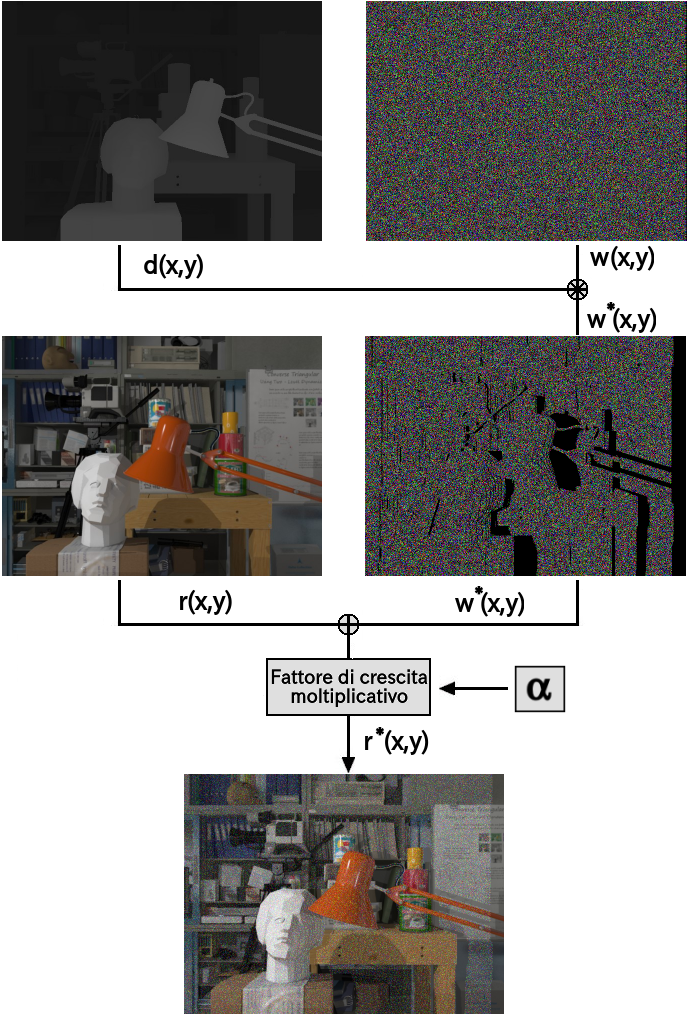
\includegraphics[width=0.9\linewidth]{./img/warp.png}
\end{figure}
\end{center}
\end{column}
\end{columns}
\end{frame}

% % % % % % % % % % FRAME % % % % % % % % % % % % %
\subsection{Processo di decodifica}
\begin{frame}[t]{\textsc{Marchiatura spaziale a disparit\`{a} coerente}}
\vspace{-2em}
\begin{columns}
\begin{column}{6cm}
	\setbeamertemplate{blocks}[rounded][shadow=false]
	\setbeamercolor{block body}{use=structure,fg=black,bg=lightgray}
\vspace{1em}
\begin{block}{Decodifica vista sinistra}
\begin{itemize}
\item Correlazione \textbf{vista sinistra} e \textbf{marchio originale}
\end{itemize}
\end{block}
\begin{block}{Decodifica vista destra}
\begin{itemize}
\item[1.] Correlazione \textbf{vista destra} e \textbf{marchio distorto}
\end{itemize}
\vspace{-0.5em}
oppure
\begin{itemize}
\item[2.] Correlazione \textbf{vista sinistra ricostruita} (attraverso vista destra e disparit\`{a}) e il marchio originale
\end{itemize}
\end{block}
\end{column}
\begin{column}{5cm}
\vspace{2em}
\begin{center}
\begin{figure}
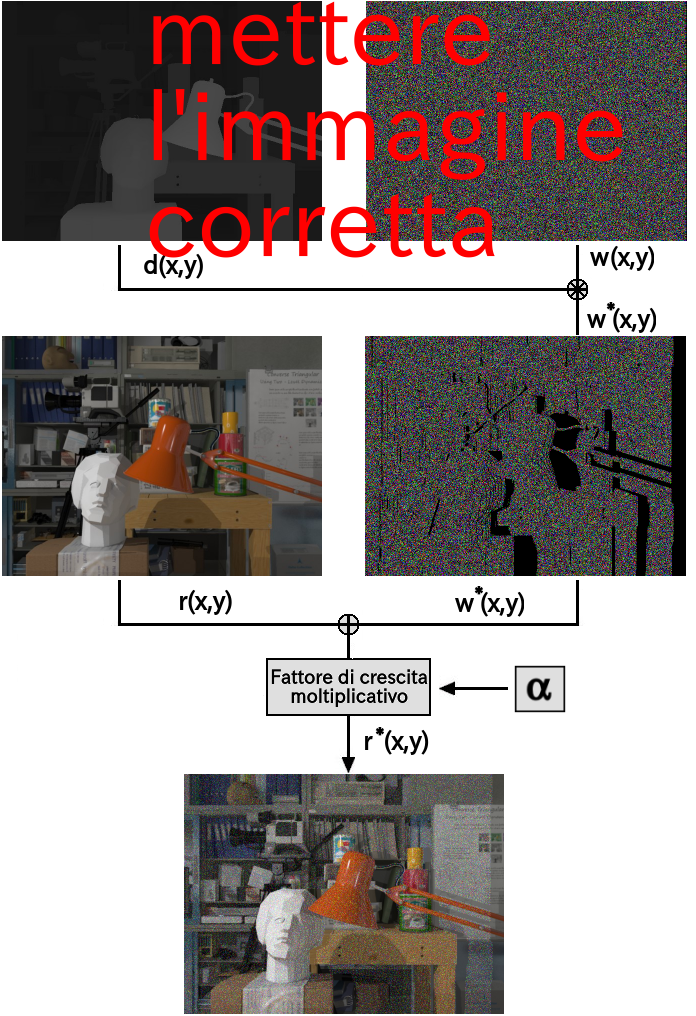
\includegraphics[width=0.9\linewidth]{./img/warp2.png}
\end{figure}
\end{center}
\end{column}
\end{columns}
\end{frame}




\end{section}

\end{document}
